% Options for packages loaded elsewhere
\PassOptionsToPackage{unicode}{hyperref}
\PassOptionsToPackage{hyphens}{url}
\PassOptionsToPackage{dvipsnames,svgnames,x11names}{xcolor}
%
\documentclass[
  letterpaper,
  DIV=11,
  numbers=noendperiod]{scrartcl}

\usepackage{amsmath,amssymb}
\usepackage{iftex}
\ifPDFTeX
  \usepackage[T1]{fontenc}
  \usepackage[utf8]{inputenc}
  \usepackage{textcomp} % provide euro and other symbols
\else % if luatex or xetex
  \usepackage{unicode-math}
  \defaultfontfeatures{Scale=MatchLowercase}
  \defaultfontfeatures[\rmfamily]{Ligatures=TeX,Scale=1}
\fi
\usepackage{lmodern}
\ifPDFTeX\else  
    % xetex/luatex font selection
\fi
% Use upquote if available, for straight quotes in verbatim environments
\IfFileExists{upquote.sty}{\usepackage{upquote}}{}
\IfFileExists{microtype.sty}{% use microtype if available
  \usepackage[]{microtype}
  \UseMicrotypeSet[protrusion]{basicmath} % disable protrusion for tt fonts
}{}
\makeatletter
\@ifundefined{KOMAClassName}{% if non-KOMA class
  \IfFileExists{parskip.sty}{%
    \usepackage{parskip}
  }{% else
    \setlength{\parindent}{0pt}
    \setlength{\parskip}{6pt plus 2pt minus 1pt}}
}{% if KOMA class
  \KOMAoptions{parskip=half}}
\makeatother
\usepackage{xcolor}
\setlength{\emergencystretch}{3em} % prevent overfull lines
\setcounter{secnumdepth}{-\maxdimen} % remove section numbering
% Make \paragraph and \subparagraph free-standing
\ifx\paragraph\undefined\else
  \let\oldparagraph\paragraph
  \renewcommand{\paragraph}[1]{\oldparagraph{#1}\mbox{}}
\fi
\ifx\subparagraph\undefined\else
  \let\oldsubparagraph\subparagraph
  \renewcommand{\subparagraph}[1]{\oldsubparagraph{#1}\mbox{}}
\fi

\usepackage{color}
\usepackage{fancyvrb}
\newcommand{\VerbBar}{|}
\newcommand{\VERB}{\Verb[commandchars=\\\{\}]}
\DefineVerbatimEnvironment{Highlighting}{Verbatim}{commandchars=\\\{\}}
% Add ',fontsize=\small' for more characters per line
\usepackage{framed}
\definecolor{shadecolor}{RGB}{241,243,245}
\newenvironment{Shaded}{\begin{snugshade}}{\end{snugshade}}
\newcommand{\AlertTok}[1]{\textcolor[rgb]{0.68,0.00,0.00}{#1}}
\newcommand{\AnnotationTok}[1]{\textcolor[rgb]{0.37,0.37,0.37}{#1}}
\newcommand{\AttributeTok}[1]{\textcolor[rgb]{0.40,0.45,0.13}{#1}}
\newcommand{\BaseNTok}[1]{\textcolor[rgb]{0.68,0.00,0.00}{#1}}
\newcommand{\BuiltInTok}[1]{\textcolor[rgb]{0.00,0.23,0.31}{#1}}
\newcommand{\CharTok}[1]{\textcolor[rgb]{0.13,0.47,0.30}{#1}}
\newcommand{\CommentTok}[1]{\textcolor[rgb]{0.37,0.37,0.37}{#1}}
\newcommand{\CommentVarTok}[1]{\textcolor[rgb]{0.37,0.37,0.37}{\textit{#1}}}
\newcommand{\ConstantTok}[1]{\textcolor[rgb]{0.56,0.35,0.01}{#1}}
\newcommand{\ControlFlowTok}[1]{\textcolor[rgb]{0.00,0.23,0.31}{#1}}
\newcommand{\DataTypeTok}[1]{\textcolor[rgb]{0.68,0.00,0.00}{#1}}
\newcommand{\DecValTok}[1]{\textcolor[rgb]{0.68,0.00,0.00}{#1}}
\newcommand{\DocumentationTok}[1]{\textcolor[rgb]{0.37,0.37,0.37}{\textit{#1}}}
\newcommand{\ErrorTok}[1]{\textcolor[rgb]{0.68,0.00,0.00}{#1}}
\newcommand{\ExtensionTok}[1]{\textcolor[rgb]{0.00,0.23,0.31}{#1}}
\newcommand{\FloatTok}[1]{\textcolor[rgb]{0.68,0.00,0.00}{#1}}
\newcommand{\FunctionTok}[1]{\textcolor[rgb]{0.28,0.35,0.67}{#1}}
\newcommand{\ImportTok}[1]{\textcolor[rgb]{0.00,0.46,0.62}{#1}}
\newcommand{\InformationTok}[1]{\textcolor[rgb]{0.37,0.37,0.37}{#1}}
\newcommand{\KeywordTok}[1]{\textcolor[rgb]{0.00,0.23,0.31}{#1}}
\newcommand{\NormalTok}[1]{\textcolor[rgb]{0.00,0.23,0.31}{#1}}
\newcommand{\OperatorTok}[1]{\textcolor[rgb]{0.37,0.37,0.37}{#1}}
\newcommand{\OtherTok}[1]{\textcolor[rgb]{0.00,0.23,0.31}{#1}}
\newcommand{\PreprocessorTok}[1]{\textcolor[rgb]{0.68,0.00,0.00}{#1}}
\newcommand{\RegionMarkerTok}[1]{\textcolor[rgb]{0.00,0.23,0.31}{#1}}
\newcommand{\SpecialCharTok}[1]{\textcolor[rgb]{0.37,0.37,0.37}{#1}}
\newcommand{\SpecialStringTok}[1]{\textcolor[rgb]{0.13,0.47,0.30}{#1}}
\newcommand{\StringTok}[1]{\textcolor[rgb]{0.13,0.47,0.30}{#1}}
\newcommand{\VariableTok}[1]{\textcolor[rgb]{0.07,0.07,0.07}{#1}}
\newcommand{\VerbatimStringTok}[1]{\textcolor[rgb]{0.13,0.47,0.30}{#1}}
\newcommand{\WarningTok}[1]{\textcolor[rgb]{0.37,0.37,0.37}{\textit{#1}}}

\providecommand{\tightlist}{%
  \setlength{\itemsep}{0pt}\setlength{\parskip}{0pt}}\usepackage{longtable,booktabs,array}
\usepackage{calc} % for calculating minipage widths
% Correct order of tables after \paragraph or \subparagraph
\usepackage{etoolbox}
\makeatletter
\patchcmd\longtable{\par}{\if@noskipsec\mbox{}\fi\par}{}{}
\makeatother
% Allow footnotes in longtable head/foot
\IfFileExists{footnotehyper.sty}{\usepackage{footnotehyper}}{\usepackage{footnote}}
\makesavenoteenv{longtable}
\usepackage{graphicx}
\makeatletter
\def\maxwidth{\ifdim\Gin@nat@width>\linewidth\linewidth\else\Gin@nat@width\fi}
\def\maxheight{\ifdim\Gin@nat@height>\textheight\textheight\else\Gin@nat@height\fi}
\makeatother
% Scale images if necessary, so that they will not overflow the page
% margins by default, and it is still possible to overwrite the defaults
% using explicit options in \includegraphics[width, height, ...]{}
\setkeys{Gin}{width=\maxwidth,height=\maxheight,keepaspectratio}
% Set default figure placement to htbp
\makeatletter
\def\fps@figure{htbp}
\makeatother

\KOMAoption{captions}{tableheading}
\makeatletter
\makeatother
\makeatletter
\makeatother
\makeatletter
\@ifpackageloaded{caption}{}{\usepackage{caption}}
\AtBeginDocument{%
\ifdefined\contentsname
  \renewcommand*\contentsname{Table of contents}
\else
  \newcommand\contentsname{Table of contents}
\fi
\ifdefined\listfigurename
  \renewcommand*\listfigurename{List of Figures}
\else
  \newcommand\listfigurename{List of Figures}
\fi
\ifdefined\listtablename
  \renewcommand*\listtablename{List of Tables}
\else
  \newcommand\listtablename{List of Tables}
\fi
\ifdefined\figurename
  \renewcommand*\figurename{Figure}
\else
  \newcommand\figurename{Figure}
\fi
\ifdefined\tablename
  \renewcommand*\tablename{Table}
\else
  \newcommand\tablename{Table}
\fi
}
\@ifpackageloaded{float}{}{\usepackage{float}}
\floatstyle{ruled}
\@ifundefined{c@chapter}{\newfloat{codelisting}{h}{lop}}{\newfloat{codelisting}{h}{lop}[chapter]}
\floatname{codelisting}{Listing}
\newcommand*\listoflistings{\listof{codelisting}{List of Listings}}
\makeatother
\makeatletter
\@ifpackageloaded{caption}{}{\usepackage{caption}}
\@ifpackageloaded{subcaption}{}{\usepackage{subcaption}}
\makeatother
\makeatletter
\@ifpackageloaded{tcolorbox}{}{\usepackage[skins,breakable]{tcolorbox}}
\makeatother
\makeatletter
\@ifundefined{shadecolor}{\definecolor{shadecolor}{rgb}{.97, .97, .97}}
\makeatother
\makeatletter
\makeatother
\makeatletter
\makeatother
\ifLuaTeX
  \usepackage{selnolig}  % disable illegal ligatures
\fi
\IfFileExists{bookmark.sty}{\usepackage{bookmark}}{\usepackage{hyperref}}
\IfFileExists{xurl.sty}{\usepackage{xurl}}{} % add URL line breaks if available
\urlstyle{same} % disable monospaced font for URLs
\hypersetup{
  pdftitle={Class 05: Data Visualization with ggplot},
  pdfauthor={Karis Kim (A16378938)},
  colorlinks=true,
  linkcolor={blue},
  filecolor={Maroon},
  citecolor={Blue},
  urlcolor={Blue},
  pdfcreator={LaTeX via pandoc}}

\title{Class 05: Data Visualization with ggplot}
\author{Karis Kim (A16378938)}
\date{}

\begin{document}
\maketitle
\ifdefined\Shaded\renewenvironment{Shaded}{\begin{tcolorbox}[enhanced, borderline west={3pt}{0pt}{shadecolor}, boxrule=0pt, sharp corners, interior hidden, frame hidden, breakable]}{\end{tcolorbox}}\fi

\renewcommand*\contentsname{Table of contents}
{
\hypersetup{linkcolor=}
\setcounter{tocdepth}{3}
\tableofcontents
}
Today we wil have our first play with the \textbf{ggplot2} package - one
of the most popular graphics packages on the planet.

There are many plotting systems in R. These include \emph{``base''}
plotting/graphics.

\begin{Shaded}
\begin{Highlighting}[]
\FunctionTok{plot}\NormalTok{(cars)}
\end{Highlighting}
\end{Shaded}

\begin{figure}[H]

{\centering 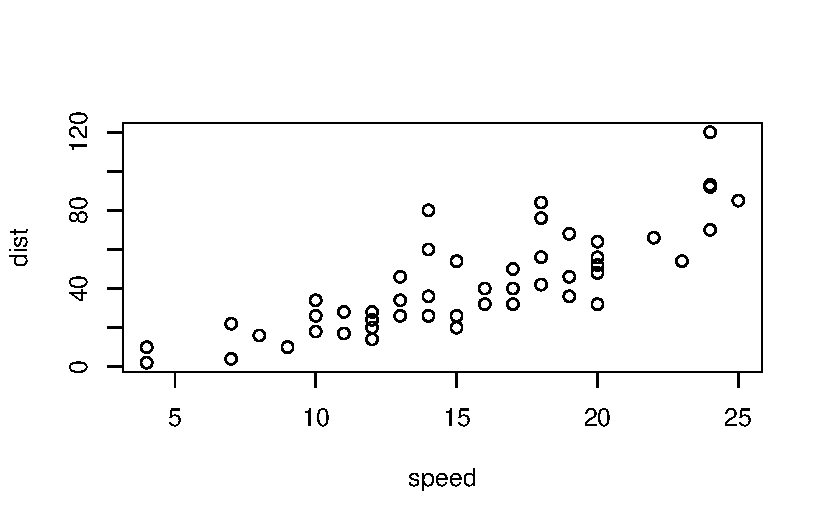
\includegraphics{Class05_files/figure-pdf/unnamed-chunk-1-1.pdf}

}

\end{figure}

Base plot is generally rather short code and somewhat dull plots - but
it is always there for you and is fast for big data sets.

If I want to use \textbf{ggplot2}, it takes some more work.

\begin{Shaded}
\begin{Highlighting}[]
\CommentTok{\# ggplot(cars)}
\end{Highlighting}
\end{Shaded}

I need to install the package first to my computer. To do this I can use
the function \texttt{install.packages("ggplot2")}

Every time I want to use the package, I need to load it up with a
\texttt{library()} call.

\begin{Shaded}
\begin{Highlighting}[]
\FunctionTok{library}\NormalTok{(ggplot2)}
\end{Highlighting}
\end{Shaded}

Now finally I can use ggplot

\begin{Shaded}
\begin{Highlighting}[]
\FunctionTok{ggplot}\NormalTok{(cars)}
\end{Highlighting}
\end{Shaded}

\begin{figure}[H]

{\centering 
\includegraphics{Class05_files/figure-pdf/unnamed-chunk-4-1.pdf}

}

\end{figure}

Every ggplot has at least 3 things:

\begin{itemize}
\tightlist
\item
  \textbf{data} (the data.frame with the data you want to plot)
\item
  \textbf{aes} (aesthetic mapping of the data to the plot)
\item
  \textbf{geom} (how do you want the plot to look, points, lines, etc.)
\end{itemize}

\begin{Shaded}
\begin{Highlighting}[]
\FunctionTok{head}\NormalTok{(cars)}
\end{Highlighting}
\end{Shaded}

\begin{verbatim}
  speed dist
1     4    2
2     4   10
3     7    4
4     7   22
5     8   16
6     9   10
\end{verbatim}

\begin{Shaded}
\begin{Highlighting}[]
\FunctionTok{ggplot}\NormalTok{(cars) }\SpecialCharTok{+}
  \FunctionTok{aes}\NormalTok{(}\AttributeTok{x=}\NormalTok{speed, }\AttributeTok{y=}\NormalTok{dist) }\SpecialCharTok{+}
  \FunctionTok{geom\_point}\NormalTok{() }\SpecialCharTok{+}
  \FunctionTok{geom\_smooth}\NormalTok{()}
\end{Highlighting}
\end{Shaded}

\begin{verbatim}
`geom_smooth()` using method = 'loess' and formula = 'y ~ x'
\end{verbatim}

\begin{figure}[H]

{\centering 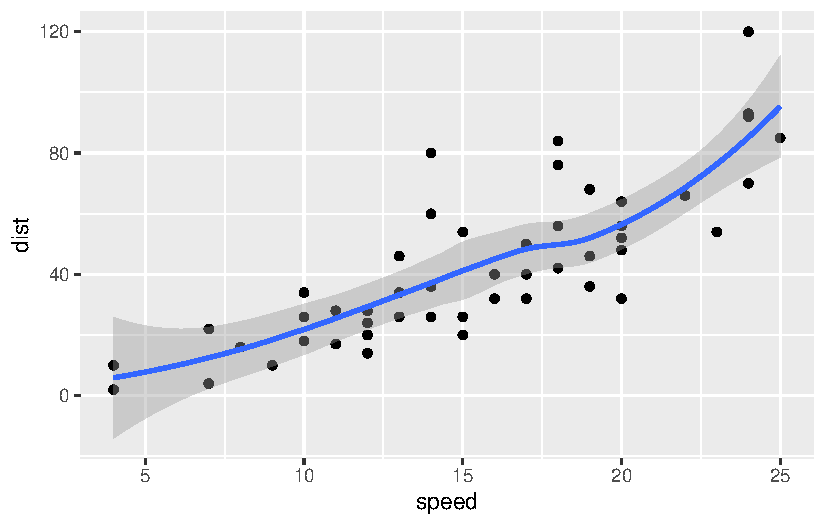
\includegraphics{Class05_files/figure-pdf/unnamed-chunk-6-1.pdf}

}

\end{figure}

I want a linear model and no standard error bounds shown on my plot. I
also want nicer axis labels, title, etc.

\begin{Shaded}
\begin{Highlighting}[]
\NormalTok{bp }\OtherTok{\textless{}{-}} \FunctionTok{ggplot}\NormalTok{(cars) }\SpecialCharTok{+}
  \FunctionTok{aes}\NormalTok{(}\AttributeTok{x=}\NormalTok{speed, }\AttributeTok{y=}\NormalTok{dist) }\SpecialCharTok{+}
  \FunctionTok{geom\_point}\NormalTok{()}
\end{Highlighting}
\end{Shaded}

\begin{Shaded}
\begin{Highlighting}[]
\NormalTok{bp }\SpecialCharTok{+} \FunctionTok{geom\_smooth}\NormalTok{(}\AttributeTok{se=}\ConstantTok{FALSE}\NormalTok{, }\AttributeTok{method=}\StringTok{"lm"}\NormalTok{) }\SpecialCharTok{+}
  \FunctionTok{labs}\NormalTok{(}\AttributeTok{title=}\StringTok{"Stopping Distance of Old Cars"}\NormalTok{,}
       \AttributeTok{x=}\StringTok{"Speed (MPH)"}\NormalTok{,}
       \AttributeTok{y=}\StringTok{"Distance (ft)"}\NormalTok{,}
       \AttributeTok{caption=}\StringTok{"From the \textasciigrave{}cars\textasciigrave{} dataset"}\NormalTok{) }\SpecialCharTok{+}
  \FunctionTok{theme\_bw}\NormalTok{()}
\end{Highlighting}
\end{Shaded}

\begin{verbatim}
`geom_smooth()` using formula = 'y ~ x'
\end{verbatim}

\begin{figure}[H]

{\centering 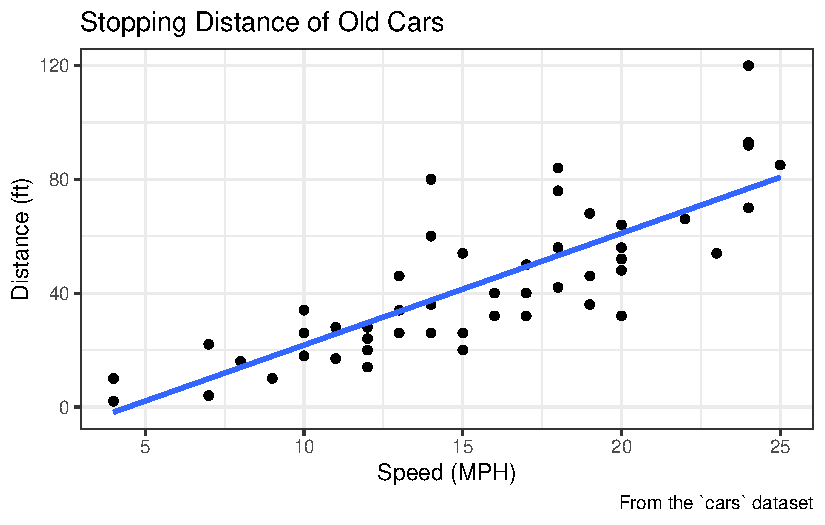
\includegraphics{Class05_files/figure-pdf/unnamed-chunk-8-1.pdf}

}

\end{figure}

\hypertarget{a-more-complicated-scatter-plot}{%
\subsection{A More Complicated Scatter
Plot}\label{a-more-complicated-scatter-plot}}

Here we make a pot of gene expression data:

\begin{Shaded}
\begin{Highlighting}[]
\NormalTok{url }\OtherTok{\textless{}{-}} \StringTok{"https://bioboot.github.io/bimm143\_S20/class{-}material/up\_down\_expression.txt"}
\NormalTok{genes }\OtherTok{\textless{}{-}} \FunctionTok{read.delim}\NormalTok{(url)}
\FunctionTok{head}\NormalTok{(genes)}
\end{Highlighting}
\end{Shaded}

\begin{verbatim}
        Gene Condition1 Condition2      State
1      A4GNT -3.6808610 -3.4401355 unchanging
2       AAAS  4.5479580  4.3864126 unchanging
3      AASDH  3.7190695  3.4787276 unchanging
4       AATF  5.0784720  5.0151916 unchanging
5       AATK  0.4711421  0.5598642 unchanging
6 AB015752.4 -3.6808610 -3.5921390 unchanging
\end{verbatim}

\begin{quote}
Q. Use the nrow() function to find out how many genes are in this
dataset. What is your answer?
\end{quote}

\begin{Shaded}
\begin{Highlighting}[]
\FunctionTok{nrow}\NormalTok{(genes)}
\end{Highlighting}
\end{Shaded}

\begin{verbatim}
[1] 5196
\end{verbatim}

\begin{quote}
Q. Use the colnames() function and the ncol() function on the genes data
frame to find out what the column names are (we will need these later)
and how many columns there are. How many columns did you find?
\end{quote}

\begin{Shaded}
\begin{Highlighting}[]
\FunctionTok{colnames}\NormalTok{(genes)}
\end{Highlighting}
\end{Shaded}

\begin{verbatim}
[1] "Gene"       "Condition1" "Condition2" "State"     
\end{verbatim}

\begin{quote}
Q. Use the table() function on the State column of this data.frame to
find out how many `up' regulated genes there are. What is your answer?
\end{quote}

\begin{Shaded}
\begin{Highlighting}[]
\FunctionTok{table}\NormalTok{(genes}\SpecialCharTok{$}\NormalTok{State)}
\end{Highlighting}
\end{Shaded}

\begin{verbatim}

      down unchanging         up 
        72       4997        127 
\end{verbatim}

\begin{quote}
Q. Using your values above and 2 significant figures. What fraction of
total genes is up-regulated in this dataset?
\end{quote}

\begin{Shaded}
\begin{Highlighting}[]
\FunctionTok{round}\NormalTok{( }\FunctionTok{sum}\NormalTok{(genes}\SpecialCharTok{$}\NormalTok{State }\SpecialCharTok{==} \StringTok{"up"}\NormalTok{) }\SpecialCharTok{/} \FunctionTok{nrow}\NormalTok{(genes) }\SpecialCharTok{*} \DecValTok{100}\NormalTok{, }\DecValTok{2}\NormalTok{) }
\end{Highlighting}
\end{Shaded}

\begin{verbatim}
[1] 2.44
\end{verbatim}

Another method to break up the values.

\begin{Shaded}
\begin{Highlighting}[]
\NormalTok{n.gene }\OtherTok{\textless{}{-}} \FunctionTok{nrow}\NormalTok{(genes)}
\NormalTok{n.up }\OtherTok{\textless{}{-}} \FunctionTok{sum}\NormalTok{(genes}\SpecialCharTok{$}\NormalTok{State }\SpecialCharTok{==} \StringTok{"up"}\NormalTok{)}

\NormalTok{up.percent }\OtherTok{\textless{}{-}}\NormalTok{ n.up}\SpecialCharTok{/}\NormalTok{n.gene }\SpecialCharTok{*} \DecValTok{100}
\FunctionTok{round}\NormalTok{(up.percent, }\DecValTok{2}\NormalTok{)}
\end{Highlighting}
\end{Shaded}

\begin{verbatim}
[1] 2.44
\end{verbatim}

\begin{Shaded}
\begin{Highlighting}[]
\FunctionTok{library}\NormalTok{(ggplot2)}
\end{Highlighting}
\end{Shaded}

\begin{Shaded}
\begin{Highlighting}[]
\NormalTok{p }\OtherTok{\textless{}{-}} \FunctionTok{ggplot}\NormalTok{(genes) }\SpecialCharTok{+}
  \FunctionTok{aes}\NormalTok{(}\AttributeTok{x=}\NormalTok{Condition1, }\AttributeTok{y=}\NormalTok{Condition2, }\AttributeTok{col=}\NormalTok{State) }\SpecialCharTok{+}
  \FunctionTok{geom\_point}\NormalTok{()}
\end{Highlighting}
\end{Shaded}

Change the Colors

\begin{Shaded}
\begin{Highlighting}[]
\NormalTok{p }\SpecialCharTok{+} \FunctionTok{labs}\NormalTok{(}\AttributeTok{title=}\StringTok{"Gene Expression Changes on Drug Treatment"}\NormalTok{,}
       \AttributeTok{x=}\StringTok{"Control (No Drug)"}\NormalTok{,}
       \AttributeTok{y=}\StringTok{"Drug Treatment"}\NormalTok{,}
       \AttributeTok{caption=}\StringTok{"From the \textasciigrave{}genes\textasciigrave{} dataset"}\NormalTok{) }\SpecialCharTok{+}
       \FunctionTok{scale\_colour\_manual}\NormalTok{( }\AttributeTok{values=}\FunctionTok{c}\NormalTok{(}\StringTok{"blue"}\NormalTok{, }\StringTok{"gray"}\NormalTok{, }\StringTok{"red"}\NormalTok{))}
\end{Highlighting}
\end{Shaded}

\begin{figure}[H]

{\centering 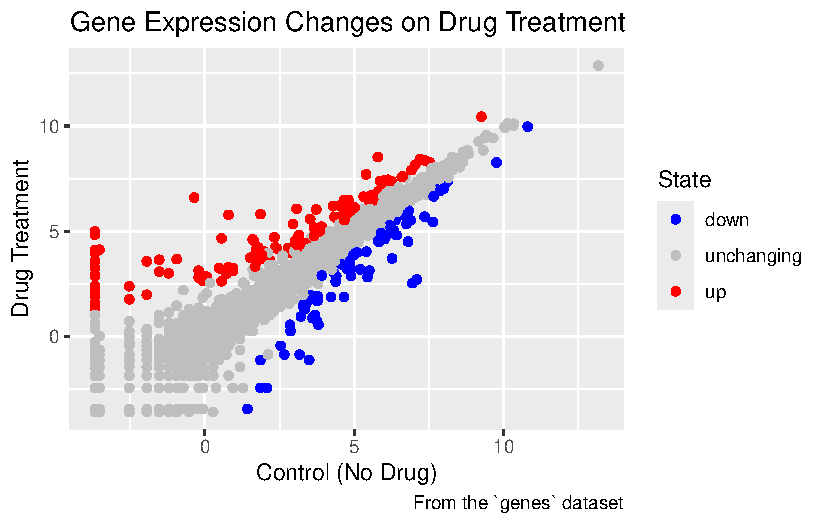
\includegraphics{Class05_files/figure-pdf/unnamed-chunk-17-1.pdf}

}

\end{figure}

\hypertarget{exploring-the-gapminder-dataset}{%
\subsection{Exploring the gapminder
Dataset}\label{exploring-the-gapminder-dataset}}

Here we will load up the gapminder dataset to get practice with
different aes mappings.

\begin{Shaded}
\begin{Highlighting}[]
\NormalTok{url }\OtherTok{\textless{}{-}} \StringTok{"https://raw.githubusercontent.com/jennybc/gapminder/master/inst/extdata/gapminder.tsv"}

\NormalTok{gapminder }\OtherTok{\textless{}{-}} \FunctionTok{read.delim}\NormalTok{(url)}
\end{Highlighting}
\end{Shaded}

\begin{quote}
Q. How many entry rows are in this dataset?
\end{quote}

\begin{Shaded}
\begin{Highlighting}[]
\FunctionTok{nrow}\NormalTok{(gapminder)}
\end{Highlighting}
\end{Shaded}

\begin{verbatim}
[1] 1704
\end{verbatim}

\begin{quote}
Q. How many columns?
\end{quote}

\begin{Shaded}
\begin{Highlighting}[]
\FunctionTok{ncol}\NormalTok{(gapminder)}
\end{Highlighting}
\end{Shaded}

\begin{verbatim}
[1] 6
\end{verbatim}

\begin{Shaded}
\begin{Highlighting}[]
\FunctionTok{dim}\NormalTok{(gapminder)}
\end{Highlighting}
\end{Shaded}

\begin{verbatim}
[1] 1704    6
\end{verbatim}

\begin{Shaded}
\begin{Highlighting}[]
\FunctionTok{head}\NormalTok{(gapminder)}
\end{Highlighting}
\end{Shaded}

\begin{verbatim}
      country continent year lifeExp      pop gdpPercap
1 Afghanistan      Asia 1952  28.801  8425333  779.4453
2 Afghanistan      Asia 1957  30.332  9240934  820.8530
3 Afghanistan      Asia 1962  31.997 10267083  853.1007
4 Afghanistan      Asia 1967  34.020 11537966  836.1971
5 Afghanistan      Asia 1972  36.088 13079460  739.9811
6 Afghanistan      Asia 1977  38.438 14880372  786.1134
\end{verbatim}

\begin{quote}
Q. How many years?
\end{quote}

\begin{Shaded}
\begin{Highlighting}[]
\FunctionTok{table}\NormalTok{(gapminder}\SpecialCharTok{$}\NormalTok{year)}
\end{Highlighting}
\end{Shaded}

\begin{verbatim}

1952 1957 1962 1967 1972 1977 1982 1987 1992 1997 2002 2007 
 142  142  142  142  142  142  142  142  142  142  142  142 
\end{verbatim}

\begin{quote}
Q. How many continents?
\end{quote}

\begin{Shaded}
\begin{Highlighting}[]
\FunctionTok{table}\NormalTok{(gapminder}\SpecialCharTok{$}\NormalTok{continent)}
\end{Highlighting}
\end{Shaded}

\begin{verbatim}

  Africa Americas     Asia   Europe  Oceania 
     624      300      396      360       24 
\end{verbatim}

I could use the \texttt{unique} function\ldots{}

\begin{Shaded}
\begin{Highlighting}[]
\FunctionTok{length}\NormalTok{( }\FunctionTok{unique}\NormalTok{(gapminder}\SpecialCharTok{$}\NormalTok{continent) )}
\end{Highlighting}
\end{Shaded}

\begin{verbatim}
[1] 5
\end{verbatim}

\begin{quote}
Q. How many countries?
\end{quote}

\begin{Shaded}
\begin{Highlighting}[]
\FunctionTok{length}\NormalTok{( }\FunctionTok{unique}\NormalTok{(gapminder}\SpecialCharTok{$}\NormalTok{country) )}
\end{Highlighting}
\end{Shaded}

\begin{verbatim}
[1] 142
\end{verbatim}

\begin{Shaded}
\begin{Highlighting}[]
\FunctionTok{ggplot}\NormalTok{(gapminder) }\SpecialCharTok{+}
  \FunctionTok{aes}\NormalTok{(}\AttributeTok{x=}\NormalTok{gdpPercap, }\AttributeTok{y=}\NormalTok{lifeExp) }\SpecialCharTok{+}
  \FunctionTok{geom\_point}\NormalTok{(}\AttributeTok{alpha=}\FloatTok{0.2}\NormalTok{)}
\end{Highlighting}
\end{Shaded}

\begin{figure}[H]

{\centering 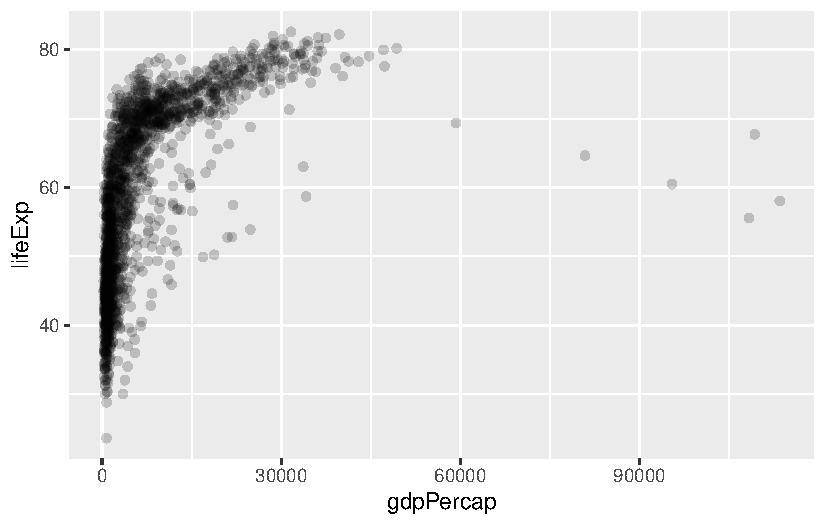
\includegraphics{Class05_files/figure-pdf/unnamed-chunk-27-1.pdf}

}

\end{figure}

\begin{Shaded}
\begin{Highlighting}[]
\FunctionTok{ggplot}\NormalTok{(gapminder) }\SpecialCharTok{+}
  \FunctionTok{aes}\NormalTok{(}\AttributeTok{x=}\NormalTok{gdpPercap, }\AttributeTok{y=}\NormalTok{lifeExp, }\AttributeTok{color=}\NormalTok{continent, }\AttributeTok{size=}\NormalTok{pop) }\SpecialCharTok{+}
  \FunctionTok{geom\_point}\NormalTok{(}\AttributeTok{alpha=}\FloatTok{0.2}\NormalTok{)}
\end{Highlighting}
\end{Shaded}

\begin{figure}[H]

{\centering 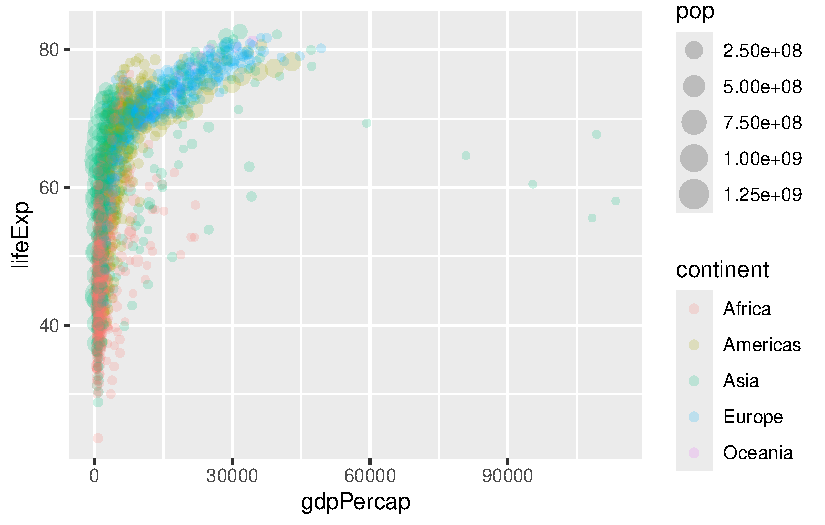
\includegraphics{Class05_files/figure-pdf/unnamed-chunk-28-1.pdf}

}

\end{figure}

\hypertarget{gapminder-2007-plot}{%
\subsubsection{Gapminder 2007 Plot}\label{gapminder-2007-plot}}

\begin{Shaded}
\begin{Highlighting}[]
\FunctionTok{library}\NormalTok{(dplyr)}
\end{Highlighting}
\end{Shaded}

\begin{verbatim}

Attaching package: 'dplyr'
\end{verbatim}

\begin{verbatim}
The following objects are masked from 'package:stats':

    filter, lag
\end{verbatim}

\begin{verbatim}
The following objects are masked from 'package:base':

    intersect, setdiff, setequal, union
\end{verbatim}

\begin{Shaded}
\begin{Highlighting}[]
\NormalTok{gapminder\_2007}\OtherTok{\textless{}{-}} \FunctionTok{filter}\NormalTok{(gapminder, year}\SpecialCharTok{==}\DecValTok{2007}\NormalTok{)}

\FunctionTok{head}\NormalTok{(gapminder\_2007)}
\end{Highlighting}
\end{Shaded}

\begin{verbatim}
      country continent year lifeExp      pop  gdpPercap
1 Afghanistan      Asia 2007  43.828 31889923   974.5803
2     Albania    Europe 2007  76.423  3600523  5937.0295
3     Algeria    Africa 2007  72.301 33333216  6223.3675
4      Angola    Africa 2007  42.731 12420476  4797.2313
5   Argentina  Americas 2007  75.320 40301927 12779.3796
6   Australia   Oceania 2007  81.235 20434176 34435.3674
\end{verbatim}

\begin{Shaded}
\begin{Highlighting}[]
\FunctionTok{ggplot}\NormalTok{(gapminder\_2007) }\SpecialCharTok{+} 
  \FunctionTok{aes}\NormalTok{(}\AttributeTok{x =}\NormalTok{ gdpPercap, }\AttributeTok{y =}\NormalTok{ lifeExp, }\AttributeTok{color=}\NormalTok{continent, }\AttributeTok{size =}\NormalTok{ pop) }\SpecialCharTok{+}
  \FunctionTok{geom\_point}\NormalTok{(}\AttributeTok{alpha=}\FloatTok{0.5}\NormalTok{)}
\end{Highlighting}
\end{Shaded}

\begin{figure}[H]

{\centering 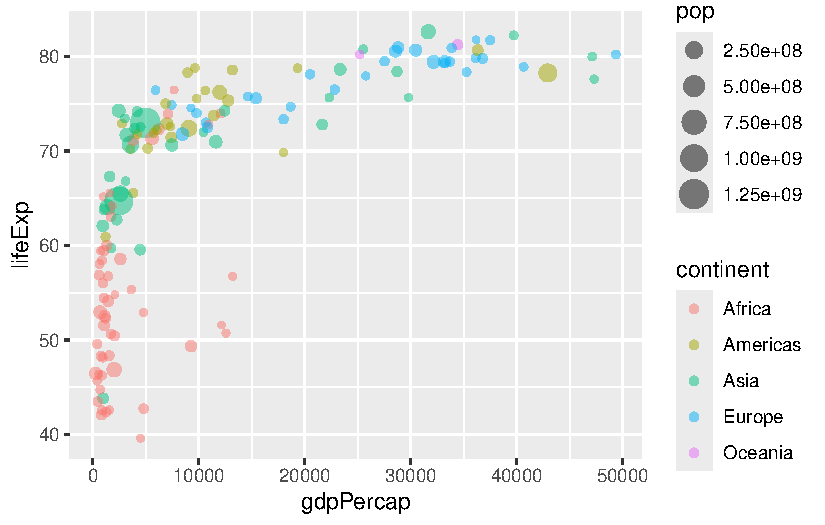
\includegraphics{Class05_files/figure-pdf/unnamed-chunk-30-1.pdf}

}

\end{figure}

\begin{Shaded}
\begin{Highlighting}[]
\FunctionTok{ggplot}\NormalTok{(gapminder) }\SpecialCharTok{+}
  \FunctionTok{aes}\NormalTok{(}\AttributeTok{x=}\NormalTok{gdpPercap, }\AttributeTok{y=}\NormalTok{lifeExp) }\SpecialCharTok{+}
  \FunctionTok{geom\_point}\NormalTok{() }\SpecialCharTok{+}
  \FunctionTok{facet\_wrap}\NormalTok{(}\SpecialCharTok{\textasciitilde{}}\NormalTok{year)}
\end{Highlighting}
\end{Shaded}

\begin{figure}[H]

{\centering 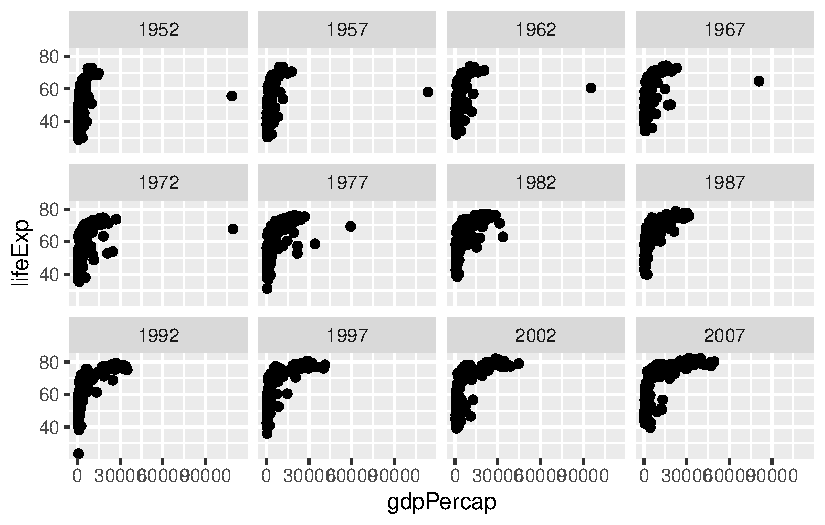
\includegraphics{Class05_files/figure-pdf/unnamed-chunk-31-1.pdf}

}

\end{figure}

\begin{Shaded}
\begin{Highlighting}[]
\NormalTok{gapminder\_1957 }\OtherTok{\textless{}{-}}\NormalTok{ gapminder }\SpecialCharTok{\%\textgreater{}\%} \FunctionTok{filter}\NormalTok{(year}\SpecialCharTok{==}\DecValTok{1957} \SpecialCharTok{|}\NormalTok{ year}\SpecialCharTok{==}\DecValTok{2007}\NormalTok{)}

\FunctionTok{ggplot}\NormalTok{(gapminder\_1957) }\SpecialCharTok{+} 
  \FunctionTok{geom\_point}\NormalTok{(}\FunctionTok{aes}\NormalTok{(}\AttributeTok{x =}\NormalTok{ gdpPercap, }\AttributeTok{y =}\NormalTok{ lifeExp, }\AttributeTok{color=}\NormalTok{continent,}
                 \AttributeTok{size =}\NormalTok{ pop), }\AttributeTok{alpha=}\FloatTok{0.7}\NormalTok{) }\SpecialCharTok{+} 
  \FunctionTok{scale\_size\_area}\NormalTok{(}\AttributeTok{max\_size =} \DecValTok{10}\NormalTok{) }\SpecialCharTok{+}
  \FunctionTok{facet\_wrap}\NormalTok{(}\SpecialCharTok{\textasciitilde{}}\NormalTok{year)}
\end{Highlighting}
\end{Shaded}

\begin{figure}[H]

{\centering 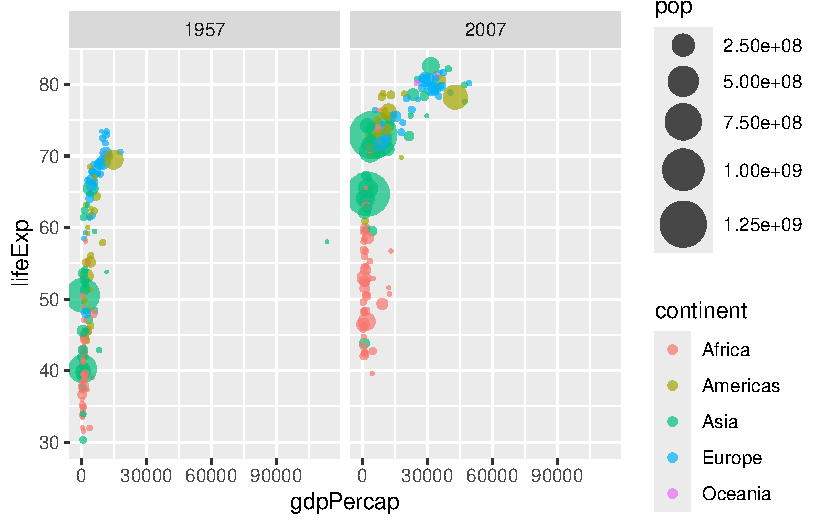
\includegraphics{Class05_files/figure-pdf/unnamed-chunk-32-1.pdf}

}

\end{figure}



\end{document}
